%%%%%%%%%%%%%%%%%%%%%%%%%%%%%%%%%%%%%%%%%
% Journal Article
% LaTeX Template
% Version 1.3 (9/9/13)
%
% This template has been downloaded from:
% http://www.LaTeXTemplates.com
%
% Original author:
% Frits Wenneker (http://www.howtotex.com)
%
% License:
% CC BY-NC-SA 3.0 (http://creativecommons.org/licenses/by-nc-sa/3.0/)
%
%%%%%%%%%%%%%%%%%%%%%%%%%%%%%%%%%%%%%%%%%

%----------------------------------------------------------------------------------------
%	PACKAGES AND OTHER DOCUMENT CONFIGURATIONS
%----------------------------------------------------------------------------------------

\documentclass[twoside]{article}

\usepackage{lipsum} % Package to generate dummy text throughout this template

\usepackage[sc]{mathpazo} % Use the Palatino font
\usepackage[T1]{fontenc} % Use 8-bit encoding that has 256 glyphs
\linespread{1.05} % Line spacing - Palatino needs more space between lines
\usepackage{microtype} % Slightly tweak font spacing for aesthetics

\usepackage[hmarginratio=1:1,top=32mm,columnsep=20pt]{geometry} % Document margins
\usepackage{multicol} % Used for the two-column layout of the document
\usepackage[hang, small,labelfont=bf,up,textfont=it,up]{caption} % Custom captions under/above floats in tables or figures
\usepackage{booktabs} % Horizontal rules in tables
\usepackage{float} % Required for tables and figures in the multi-column environment - they need to be placed in specific locations with the [H] (e.g. \begin{table}[H])
\usepackage{hyperref} % For hyperlinks in the PDF

\usepackage{lettrine} % The lettrine is the first enlarged letter at the beginning of the text
\usepackage{paralist} % Used for the compactitem environment which makes bullet points with less space between them

\usepackage{abstract} % Allows abstract customization
\renewcommand{\abstractnamefont}{\normalfont\bfseries} % Set the "Abstract" text to bold
\renewcommand{\abstracttextfont}{\normalfont\small\itshape} % Set the abstract itself to small italic text

\usepackage{titlesec} % Allows customization of titles
\renewcommand\thesection{\Roman{section}} % Roman numerals for the sections
\renewcommand\thesubsection{\Roman{subsection}} % Roman numerals for subsections
\titleformat{\section}[block]{\large\scshape\centering}{\thesection.}{1em}{} % Change the look of the section titles
\titleformat{\subsection}[block]{\large}{\thesubsection.}{1em}{} % Change the look of the section titles

\usepackage{fancyhdr} % Headers and footers
\pagestyle{fancy} % All pages have headers and footers
\fancyhead{} % Blank out the default header
\fancyfoot{} % Blank out the default footer
\fancyhead[C]{Running title $\bullet$ May 2017 $\bullet$ Vol. I, No. 1} % Custom header text
\fancyfoot[RO,LE]{\thepage} % Custom footer text

\usepackage{graphicx}
%----------------------------------------------------------------------------------------
%	TITLE SECTION
%----------------------------------------------------------------------------------------

\title{\vspace{-15mm}\fontsize{24pt}{10pt}\selectfont\textbf{Version Control System}\\
\Large(Introduction to Git)\\
\large\emph{Maulana Abul Kalam Azad University of Technology (Formerly WBUT)}} % Article title

\author{
\large
\textsc{Rohit Das}%\thanks{A thank you or further information}
\\[2mm] % Your name
\normalsize 30000114022 \\ % Your institution
\normalsize {rohit.das950@gmail.com}\\\\% Your email address
\vspace{-5mm}
\large
\textsc{Rudra Nil Basu}%\thanks{A thank you or further information}
\\[2mm]\\ % Your name
\normalsize 30000114023 \\ % Your institution
\normalsize{rudra.nil.basu@gmail.com} % Your email address
\vspace{-5mm}
}

\date{}

%----------------------------------------------------------------------------------------

\begin{document}

\maketitle % Insert title

\thispagestyle{fancy} % All pages have headers and footers

%----------------------------------------------------------------------------------------
%	ABSTRACT
%----------------------------------------------------------------------------------------

\begin{abstract}

\noindent{Version control has been an essential aspect of any
software development project since early 1980s. In the recent
years, however, we see version control as a common feature
embedded in many collaborative based software packages; such
as word processors, spreadsheets and wikis. In this paper, we
explain the common structure of version control systems,
provide historical information on their development, and
identify future improvements. } 
%\lipsum[1] % Dummy abstract text

\end{abstract}

%----------------------------------------------------------------------------------------
%	ARTICLE CONTENTS
%----------------------------------------------------------------------------------------

\begin{multicols}{2} % Two-column layout throughout the main article text

\section{Synopsis}

\lettrine[nindent=0em,lines=3]{T}his chapter will be about getting started with VCS using Git. We will begin by explaining some background on version control tools, then move on to how to get Git running on our system and finally how to get it set up to start working with. At the end of this report we should understand why Git is around, why you should use it and we should be all set up to do so.



%------------------------------------------------

\section{Introduction}

\lettrine[nindent=0em,lines=3]{W}hat is "version control", and why should we care? Version control is a system that records changes to a file or set of files over time so that we can recall specific versions later. 

If a graphic or web designer wants to keep every version of an image or layout (which he/she would most certainly want to), a Version Control System (VCS) is a very wise thing to use. It allows us to revert files back to a previous state, revert the entire project back to a previous state, compare changes over time, see who last modified something that might be causing a problem, who introduced an issue and when, and more. Using a VCS also generally means that if we screw things up or lose files, we can easily recover. In addition, we get all this for very little overhead.
%\lipsum[2-3] % Dummy text

%------------------------------------------------

\section{Benefits}

\lettrine[nindent=0em,lines=3]{D}eveloping software without using version control is risky, like not having backups. Version control can also enable developers to move faster and it allows software teams to preserve efficiency and agility as the team scales to include more developers.

Version Control Systems (VCS) have seen great improvements over the past few decades and some are better than others.One of the most popular VCS tools in use today is called Git. Git is a Distributed VCS, a category known as DVCS.Like many of the most popular VCS systems available today, Git is free and open source. Regardless of what they are called, or which system is used, the primary benefits you should expect from version control are as follows.
\begin{compactitem}
\item A complete long-term change history of every file. This means every change made by many individuals over the years. Changes include the creation and deletion of files as well as edits to their contents. This history should also include the author, date and written notes on the purpose of each change. Having the complete history enables going back to previous versions to help in root cause analysis for bugs and it is crucial when needing to fix problems in older versions of software. If the software is being actively worked on, almost everything can be considered an "older version" of the software.
\item \textbf{Branching and merging.} Having team members work concurrently is a no-brainer, but even individuals working on their own can benefit from the ability to work on independent streams of changes. Creating a "branch" in VCS tools keeps multiple streams of work independent from each other while also providing the facility to merge that work back together, enabling developers to verify that the changes on each branch do not conflict. There are many different workflows that teams can choose from when they decide how to make use of branching and merging facilities in VCS.

\item \textbf{Traceability.} Being able to trace each change made to the software and connect it to project management and bug tracking software such as JIRA, and being able to annotate each change with a message describing the purpose and intent of the change can help not only with root cause analysis and other forensics. Having the annotated history of the code at your fingertips when you are reading the code, trying to understand what it is doing and why it is so designed can enable developers to make correct and harmonious changes that are in accord with the intended long-term design of the system. This can be especially important for working effectively with legacy code and is crucial in enabling developers to estimate future work with any accuracy.\\
\end{compactitem}

While it is possible to develop software without using any version control, doing so subjects the project to a huge risk that no professional team would be advised to accept. So the question is not whether to use version control but which version control system to use.

There are many choices, but here we are going to focus on just one, Git.


%\lipsum[4] % Dummy text

%------------------------------------------------

\section{Graph Structure}

\lettrine[nindent=0em,lines=3]{I}n terms of graph theory, revisions are generally thought of as a line of development (the trunk) with branches off of this, forming a directed tree, visualized as one or more parallel lines of development (the "mainlines" of the branches) branching off a trunk. In reality the structure is more complicated, forming a directed acyclic graph, but for many purposes "tree with merges" is an adequate approximation.

Revisions occur in sequence over time, and thus can be arranged in order, either by revision number or timestamp. Revisions are based on past revisions, though it is possible to largely or completely replace an earlier revision, such as "delete all existing text, insert new text". In the simplest case, with no branching or undoing, each revision is based on its immediate predecessor alone, and they form a simple line, with a single latest version, the "HEAD" revision or tip. In graph theory terms, drawing each revision as a point and each "derived revision" relationship as an arrow (conventionally pointing from older to newer, in the same direction as time), this is a linear graph. If there is branching, so multiple future revisions are based on a past revision, or undoing, so a revision can depend on a revision older than its immediate predecessor, then the resulting graph is instead a directed tree (each node can have more than one child), and has multiple tips, corresponding to the revisions without children ("latest revision on each branch"). In principle the resulting tree need not have a preferred tip ("main" latest revision) - just various different revisions - but in practice one tip is generally identified as HEAD. When a new revisions is based on HEAD, it is either identified as the new HEAD, or considered a new branch. The list of revisions from the start to HEAD (in graph theory terms, the unique path in the tree, which forms a linear graph as before) is the trunk or mainline. Conversely, when a revision can be based on more than one previous revision (when a node can have more than one parent), the resulting process is called a merge, and is one of the most complex aspects of revision control. This most often occurs when changes occur in multiple branches (most often two, but more are possible), which are then merged into a single branch incorporating both changes. If these changes overlap, it may be difficult or impossible to merge, and require manual intervention or rewriting.

In the presence of merges, the resulting graph is no longer a tree, as nodes can have multiple parents, but is instead a rooted directed acyclic graph (DAG). The graph is acyclic since parents are always backwards in time, and rooted because there is an oldest version. However, assuming that there is a trunk, merges from branches can be considered as "external" to the tree - the changes in the branch are packaged up as a patch, which is applied to HEAD (of the trunk), creating a new revision without any explicit reference to the branch, and preserving the tree structure. Thus, while the actual relations between versions form a DAG, this can be considered a tree plus merges, and the trunk itself is a line.

In distributed revision control, in the presence of multiple repositories these may be based on a single original version (a root of the tree), but there need not be an original root, and thus only a separate root (oldest revision) for each repository, for example if two people starting working on a project separately. Similarly in the presence of multiple data sets (multiple projects) that exchange data or merge, there isn't a single root, though for simplicity one may think of one project as primary and the other as secondary, merged into the first with or without its own revision history.
%\lipsum[5] % Dummy text
\begin{figure}[H]
\centering
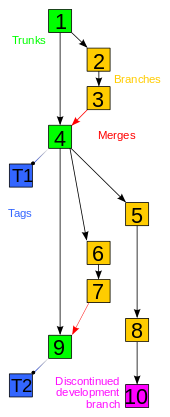
\includegraphics[width=125pt,height=\textheight,keepaspectratio]{/home/mouri/Documents/LaTeX-files/semi_repo/git1.png}
\end{figure}
%\begin{equation}
%\label{eq:emc}
%e = mc^2
%\end{equation}

%\lipsum[6] % Dummy text

%------------------------------------------------

\section{Categorizing Version-Control Systems}
\lettrine[nindent=0em,lines=3]{T}here are three fundamental ways ways in which VCSes can differ from each other. They can be centralized or decentralized; they can be locking, merge-before-commit, or commit-before-merge; and they can do file operations or fileset operations.

In second- and third-generation systems, there are two subtler sets of issues. Some VCSes are snapshot-based and some are changeset-based. Some have container identity and other do not.

\subsection{Centralized vs. Decentralized}

Early VCSes were designed around a centralized model in which each project has only one repository used by all developers. All “document management systems” are designed this way. This model has two important problems. One is that a single repository is a single point of failure — if the repository server is down all work stops. The other is that you need to be connected live to the server to do checkins and checkouts; if you're offline, you can't work.

The very earliest first-generation VCSes supported local access only; that is, all developers of a project needed to be on the same machine as the single central project repository. Second-generation VCSes, while still centralizing each project around a single repository, supported a client-server model allowing developers to work with it over a network from other machines.

Newer, third-generation VCSes are decentralized. A project may have several different repositories, and these systems support a sort of super-merge between repositories that tries to reconcile their change histories. At the limit, each developer has his/her own repository, and repository merges replace checkin/commit operations as a way of passing code between developers.

An important practical benefit is that such systems support disconnected operation; you don't need to be on the Internet to commit to the repository because you carry your own repository around with you. Pushing changesets to someone else's repository is a slower but also less frequent operation.
%\lipsum[7] % Dummy text

\subsection{Conflict resolution}
A version control system must have some mechanism to prevent or resolve conflicts among users who want to change the same file. There are three distinct ways to accomplish this.

\subsubsection{Locking}
With version-control locking, workfiles are normally read-only so that you cannot change them. You ask the VCS to make a work file writable for you by locking it; only one user can do this at any given time. When you check in your changes, that unlocks the file, making the work file read-only again. This allows other users to lock the file to make further changes.

\subsubsection{Merge before commit}
In a merge-before-commit system, the VCS notices when you are attempting a commit against a file or files that have changed since you started editing, and requires you to resolve the conflict before you can complete the commit.
%\lipsum[8] % Dummy text
\subsubsection{Commit before merge}
It is possible to design a VCS so it never blocks a commit. Instead, if the repository copy has changed since the files(s) were checked out, the commit can simply be shunted to a new branch. Subsequently, the branches may remain separate; or, any developer may perform a merge that brings them back together.

\subsection{File versus fileset operations.}
In early VCSes, some of which are still in use today, checkins and other operations are file-based; each file has its own master file with its own comment- and revision history separate from that of all other files in the system. Later systems do fileset operations; most importantly, a checkin may include changes to several files and that change set is treated as a unit by the system. Any comment associated with the change doesn't belong to any one file, but is attached to the combination of that fileset and its revision number.

Filesets are necessary; when a change to multiple files has to be backed out, it's important to be able to easily identify and remove all of it. But it took some years for designers to figure that out, and while file-based systems are passing out of use there are lots of legacy repositories using file-centric VCSes still to be dealt with at time of writing in early 2008.

\subsection{Container identity.}
In a VCS with container identity, files and directories have a stable internal identity, initialized when the file is added to the repository. This identity follows them through renames and moves. This means that filenames and directories are versioned, so that it is possible (for example) for the VCS to notice while doing a merge between branches that two files with different names are descendants of the same file and do a smarter merge of their contents.

Container identity can be implemented by giving each file in the repository a “true name” analogous to a Unix inode, Alternatively, it can be implemented implicitly by keeping all records of renames in history and chasing through them each time the VCS needs to check what file X was called in revision Y.

Absence of container identity has the symptom that file rename/move operations have to be modeled as a file add followed by a delete, with the deleted file's history magically copied during the add.

Usually VCSes that lack container identity also create parent directories on the fly whenever a file is added or checked out, and you cannot actually have an empty directory in a repository.

%------------------------------------------------

\section{Future Prospects}
Despite the idea that version control systems have been used since before the development of computers, most users did not know how to use such systems to their complexity. More recently, though, these tools have become simple, efficient, and accessible to most users.

A great contribution to the popularization of such technology has been made by Apple and its Time Machine. Most users are unaware of how exactly this tool works, but the result it delivers is extremely useful and effortlessly achieved by the user.

Version control systems for designers, musicians and developers use a common technology and differ only in their appearance for different users and tasks. In the near future, version control tools will be a standard part of the working process and user interface. It is difficult to imagine a world without version control. These systems store versions of a work and allow multiple users to access any part of a project from different locations on the planet, using different devices and even using different programs.

Since such systems maintain the independent activity of an entire team, large companies will be able to collaborate interdepartmentally. Developers will have access to the latest version of the project at all times. It allows for greater efficiency by removing the need for developers to learn design programs and does not rely on designers to confirm changes made by programmers. Changes in design will automatically be delivered in your code. It does not matter what program the user is working with because the common mechanisms are hidden in its depths.


%----------------------------------------------------------------------------------------
%	REFERENCE LIST
%----------------------------------------------------------------------------------------

\begin{thebibliography}{99} % Bibliography - this is intentionally simple in this template
 
\bibitem[O'Sullivan, Bryan (2009)]{O'Sullivan, Bryan (2009)}
Sebastopol: O'Reilly Media, Inc. ISBN 9780596555474. Retrieved 4 September 2015.
\newblock Mercurial: the Definitive Guide.
 
\bibitem[Wheeler, David]{.}
Retrieved May 8, 2007.
\newblock Comments on Open Source Software / Free Software (OSS/FS) Software Configuration Management (SCM) Systems".
\bibitem[Spolsky, Joel (2010-03-17)]{.}
Retrieved 2010-06-18.
\newblock "Distributed Version Control is here to stay, baby". Joel on Software.
\bibitem[Eric Raymond]{.}
http://www.catb.org/esr/writings/version-control/version-control.html\\
\newblock Understanding Version-Control Systems (DRAFT)
\end{thebibliography}

\begin{figure}[H]
\centering

\includegraphics[width=135pt,height=\textheight,keepaspectratio]{/home/mouri/Documents/LaTeX-files/semi_repo/git2.png}
\end{figure}


%----------------------------------------------------------------------------------------

\end{multicols}

\end{document}
